\documentclass[tikz,border=0pt]{standalone}
\usepackage{graphicx}
\usepackage{amsmath,amssymb}
\usepackage{times}

\begin{document}
\begin{tikzpicture}[x=1bp,y=1bp]
  \path[use as bounding box] (0,0) rectangle (1020,432);
  \node[anchor=south west,inner sep=0] at (0,0) {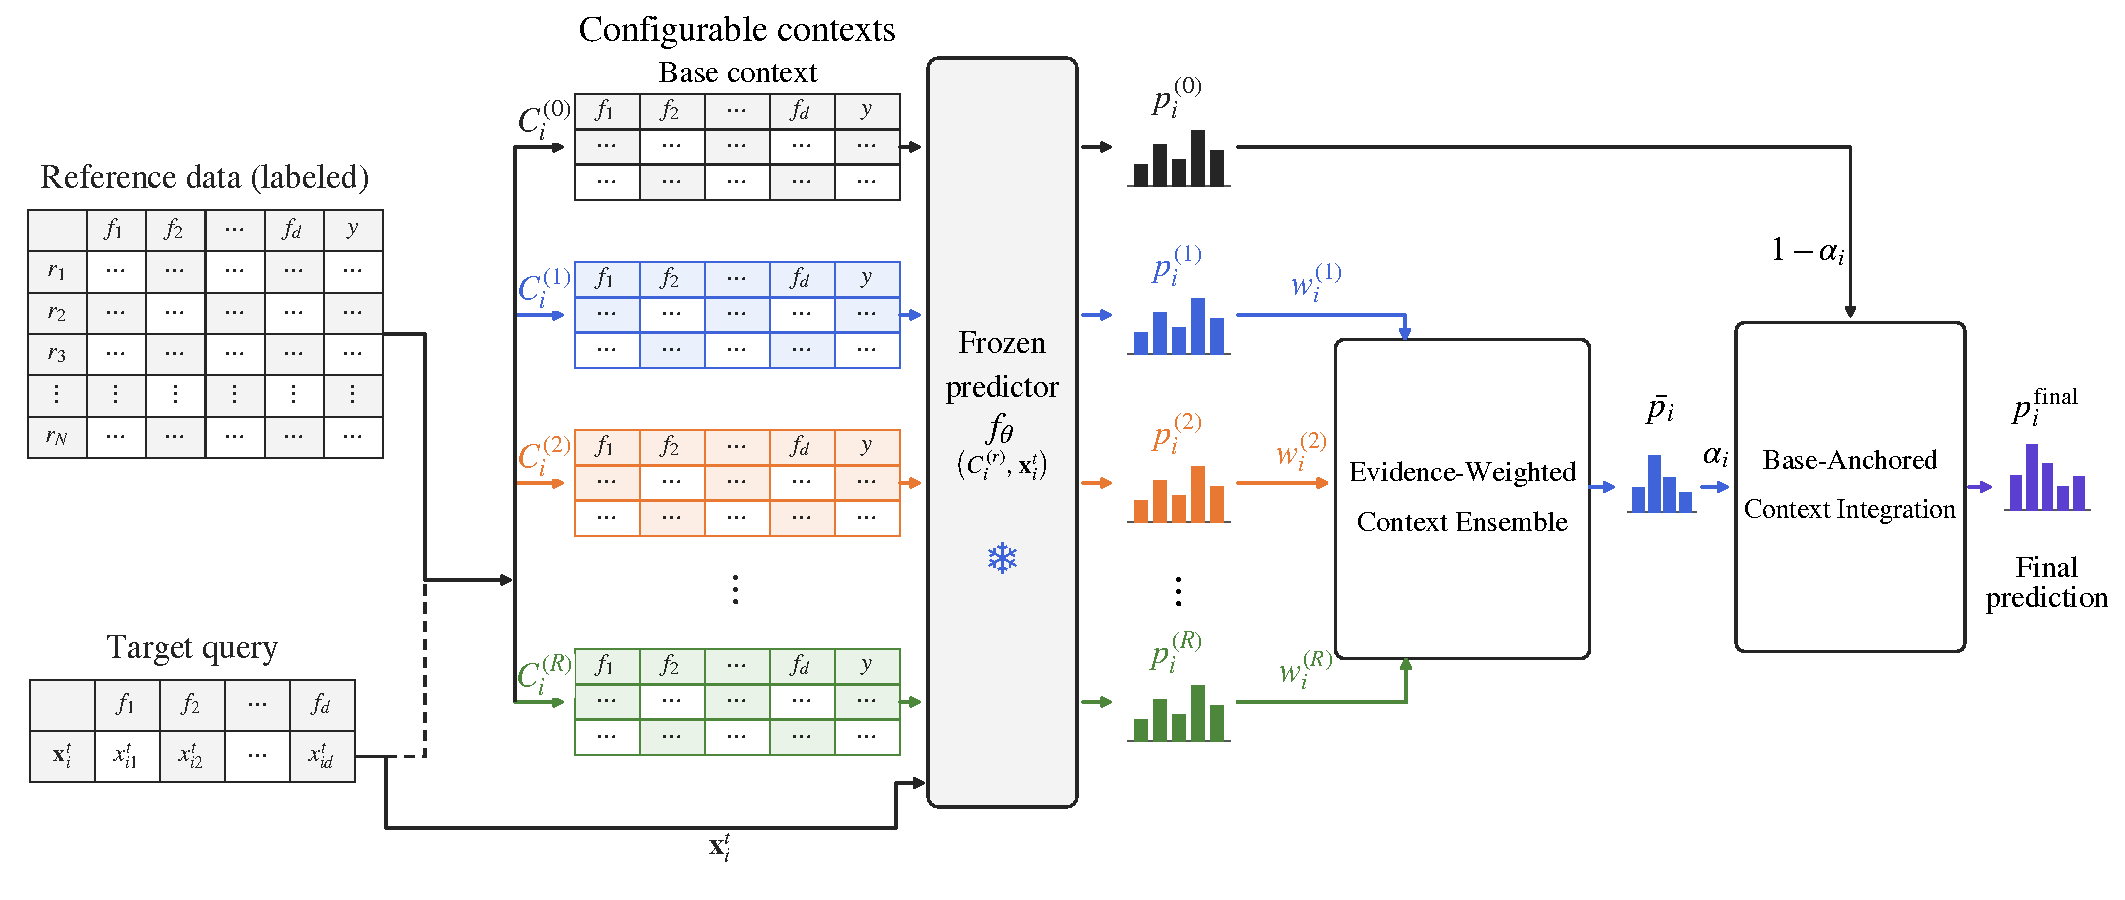
\includegraphics{context_ensemble_framework_pfn_input_semantics_fixed_lines.pdf}};

  % The published notation uses t for target queries and keeps Base separate.
  \fill[white] (244,365) rectangle (278,390);
  \node[anchor=center,inner sep=0,font=\fontsize{13}{14}\selectfont]
    at (261,377.5) {$C^{(0)}$};

  % The input panel represents the target batch while highlighting the query.
  \fill[white] (34,109) rectangle (162,137);
  \node[anchor=center,inner sep=0,font=\fontsize{9.2}{10.2}\selectfont]
    at (98,126) {Unlabeled target batch $\mathcal X_t$};
  \node[anchor=center,inner sep=0,font=\fontsize{8.3}{9.2}\selectfont]
    at (98,115.5) {(current query $x_i^t$)};

  \fill[white] (14,54) rectangle (169,80);
  \draw[line width=0.45bp] (14,54) rectangle (169,80);
  \foreach \x in {46,77,108,139} {\draw[line width=0.45bp] (\x,54)--(\x,80);}
  \node[anchor=center,inner sep=0,font=\fontsize{8.4}{9}\selectfont] at (30,67) {$\mathbf{x}_i^t$};
  \node[anchor=center,inner sep=0,font=\fontsize{8.4}{9}\selectfont] at (61.5,67) {$x_{i1}^t$};
  \node[anchor=center,inner sep=0,font=\fontsize{8.4}{9}\selectfont] at (92.5,67) {$x_{i2}^t$};
  \node[anchor=center,inner sep=0,font=\fontsize{8.4}{9}\selectfont] at (123.5,67) {$\cdots$};
  \node[anchor=center,inner sep=0,font=\fontsize{8.4}{9}\selectfont] at (154.5,67) {$x_{id}^t$};

  \fill[white] (329,16) rectangle (359,39);
  \node[anchor=center,inner sep=0,font=\fontsize{11}{12}\selectfont]
    at (344,27.5) {$x_i^t$};

  \fill[white] (445,199) rectangle (510,223);
  \node[anchor=center,inner sep=0,font=\fontsize{8.6}{9.4}\selectfont]
    at (477.5,211) {$(C_i^{(r)},x_i^t)$};

  % The integration coefficient is query dependent in the method definition.
  \fill[white] (846,304) rectangle (887,324);
  \node[anchor=center,inner sep=0,font=\fontsize{13}{14}\selectfont]
    at (866.5,314) {$1-\alpha_i$};
  \fill[white] (814,207) rectangle (831,224);
  \node[anchor=center,inner sep=0,font=\fontsize{12}{13}\selectfont]
    at (822.5,215.5) {$\alpha_i$};
\end{tikzpicture}
\end{document}
